\documentclass[a4paper,14pt]{extreport}
\usepackage[left=1.5cm,right=1.5cm,
    top=1.5cm,bottom=2cm,bindingoffset=0cm]{geometry}
\usepackage{scrextend}
\usepackage[T1,T2A]{fontenc}
\usepackage[utf8]{inputenc}
\usepackage[english,russian,ukrainian]{babel}
\usepackage{tabularx}
\usepackage{amssymb}
\usepackage{color}
\usepackage{amsmath}
\usepackage{mathrsfs}
\usepackage{listings}
\usepackage{graphicx}
\graphicspath{ {./images/} }
\usepackage{lipsum}
\usepackage{xcolor}
\usepackage{hyperref}
\usepackage{tcolorbox}
\usepackage{tikz}
\usepackage[framemethod=TikZ]{mdframed}
\usepackage{wrapfig,boxedminipage,lipsum}
\mdfdefinestyle{MyFrame}{%
linecolor=blue,outerlinewidth=2pt,roundcorner=20pt,innertopmargin=\baselineskip,innerbottommargin=\baselineskip,innerrightmargin=20pt,innerleftmargin=20pt,backgroundcolor=gray!50!white}
 \usepackage{csvsimple}
 \usepackage{supertabular}
\usepackage{pdflscape}
\usepackage{fancyvrb}
%\usepackage{comment}
\usepackage{array,tabularx}
\usepackage{colortbl}

\usepackage{varwidth}
\tcbuselibrary{skins}
\usepackage{fancybox}


\usepackage{tikz}
\usepackage[framemethod=TikZ]{mdframed}
\usepackage{xcolor}
\usetikzlibrary{calc}
\makeatletter
\newlength{\mylength}
\xdef\CircleFactor{1.1}
\setlength\mylength{\dimexpr\f@size pt}
\newsavebox{\mybox}
\newcommand*\circled[2][draw=blue]{\savebox\mybox{\vbox{\vphantom{WL1/}#1}}\setlength\mylength{\dimexpr\CircleFactor\dimexpr\ht\mybox+\dp\mybox\relax\relax}\tikzset{mystyle/.style={circle,#1,minimum height={\mylength}}}
\tikz[baseline=(char.base)]
\node[mystyle] (char) {#2};}
\makeatother

\definecolor{ggreen}{rgb}{0.4,1,0}
\definecolor{rred}{rgb}{1,0.1,0.1}
\definecolor{amber}{rgb}{1.0, 0.75, 0.0}
\definecolor{babyblue}{rgb}{0.54, 0.81, 0.94}
\definecolor{asparagus}{rgb}{0.53, 0.66, 0.42}
\definecolor{chartreuse}{rgb}{0.5, 1.0, 0.0}
\definecolor{darkorchid}{rgb}{0.6, 0.2, 0.8}

\usepackage{float}
\usepackage{wrapfig}
\usepackage{framed}
%for nice Code{
\lstdefinestyle{customc}{
  belowcaptionskip=1\baselineskip,
  breaklines=true,
  frame=L,
  xleftmargin=\parindent,
  language=C,
  showstringspaces=false,
  basicstyle=\small\ttfamily,
  keywordstyle=\bfseries\color{green!40!black},
  commentstyle=\itshape\color{purple!40!black},
  identifierstyle=\color{blue},
  stringstyle=\color{orange},
}
\lstset{escapechar=@,style=customc}
%}


\begin{document}
\pagecolor{white}

%----------------------------------------1
\newtcbox{\xmybox}[1][red]{on line, arc=7pt,colback=#1!10!white,colframe=#1!50!black, before upper={\rule[3pt] {0pt}{10pt}},boxrule=1pt,boxsep=0pt,left=6pt,right=6pt,top=2pt,bottom=2pt}


\begin{center}Bohdan Lyshchenko DP-82 Variant №4
\vspace{1cm}

\end{center}


\begin{center}Перелікуйте і поясніть основні об’ємні і поверхневі пружні хвилі.\end{center}

Elastic waves can be described in the elastic continuum approximation. Consider the oscillations of the elementary volume taken inside a crystal in the form of a cube
$ \triangle x \triangle y \triangle z $. The mass of this cube is equal to the product of its volume and density: $ m = \rho \triangle V = \rho \triangle x \triangle y
\triangle z $. The acceleration d2x / dt2, which corresponds to the previously mentioned model of the oscillator, is determined by the second time derivative of the deformation component x1: dx21 / dt2 (for simplification, consider oscillations only along one direction - along the x-axis). \\

The elastic force Fx (component of the force along the x-axis) can be calculated using a model that compares the stresses on the two faces of the cube: X1 (x) and X1
$ \triangle x $). Their difference can be decomposed into a series in which to leave only the first member of the series (linear approximation):

$$
X_{1}(x+\Delta x)-X_{1}(x)=\frac{\partial X}{\partial x} \Delta x
$$
The resulting force is equal to the voltage difference multiplied by the area normal to the operating voltage:
$$
F_{x}=\left[\frac{\partial X}{\partial x} \Delta x\right] \Delta y \Delta z
$$
Other forces $ \left (\partial X_ {2} / \partial y_ {1} \partial X_ {3} / \partial z \right) $ also act in the considered elementary cube in the direction of displacement $ x_ {1} $ i due to changes within the elementary volume of stresses $ X_ {2} \mathrm {i} X_ {3} $ (in Fig. 6.5, and these components of forces are not shown). Similar equations can be obtained for the deformation waves: $ x_ {2} $ and $ x_ {3}. $ Substituting the results into the oscillator equation, we obtain
$$
\rho \frac{d^{2} x}{d t^{2}}=\frac{\partial X_{1}}{\partial x}+\frac{\partial X_{2}}{\partial y}+\frac{\partial X_{3}}{\partial z}
$$
The solutions of the consolidated equation depend on the specific symmetry of whether
another crystal or texture, because they are determined by a set of components of the matrix. For a relatively simple case Centrosymmetric

$$
x=x_{0} \exp [i(\omega t-K x)]
$$
leads to the following dispersion ratio:
$$
\omega^{2} \rho=c_{11} K^{2}, \omega=\sqrt{c_{11} / \rho} K
$$
In contrast to the similar discrete "atomic chain", where the dispersion law $ \omega (K): \omega = 2 \sqrt {c / m} \sin (Ka / 2) $, in the approximation of the elastic continuum, when the discreteness of the structure is not taken into account , spatial dispersion does not occur:
The frequency of elastic waves does not depend on the frequency. Longitudinal velocity
waves along the direction [100] in cubic crystals depends only on the density of the crystal and one of the components of elastic stiffness:
$$
Q_{L A[100]}=\omega / K=\sqrt{c_{11} / \rho}
$$

The most common cases of surface waves include the following: \\

1. Rayleigh waves propagating along the boundary of an elastic half-space with a vacuum (or with a sufficiently rarefied gaseous medium). Phase velocity of Rayleigh waves $ \delta $ R $ \approx \delta $ 0.9 $ \delta $ T, where $ \delta $ T is the phase velocity of a plane transverse wave. The phase velocity of such waves is directed parallel to the surface, and the oscillating particles of the medium near it have both transverse, perpendicular to the surface and longitudinal components of the displacement vector. These particles describe in their oscillations elliptical trajectories in a plane perpendicular to the surface, and passing through the direction of the phase velocity. This plane is called the sagittal. \\

2. Attenuating waves of the Rayleigh type, existing at the boundary of a solid with a liquid. Naturally, elastic surface waves cannot exist in an unstressed liquid. However, it should be noted that at the frequencies of the ultrasonic range in the real liquid can still occur surface waves, for which the determining factor is not elastic forces, and surface tension (so-called capillary waves). If a solid is adjacent to a liquid, and the speed of sound in a liquid is less than the speed of sound $ \delta $ sv in a solid (this is true for almost all real media), then at the boundary of a solid and a liquid a damped Rayleigh wave may propagate. \\

3. Non-extinguishing waves with vertical polarization, propagating on the boundary between liquid and solid. The speed of sound in a liquid is less than the speed of sound in a solid, and therefore an undamped wave in a solid coexists with a damped one. It propagates along the boundary of media with a phase velocity less than the velocity of the $ \delta $ kind of wave in the liquid and the velocity of the longitudinal $ \delta $ L and transverse $ \delta $ T waves in the solid.

4. Stoneley waves propagating along the flat boundary of two solid media, the modulus of elasticity and density of which do not differ much.
The Stoneley wave consists of two Rayleigh waves (one in each medium). The phase velocity of Stoneley waves is less than the velocities of longitudinal $ \delta $ L and transverse $ \delta $ T in both boundary media. The vertical and horizontal components of the displacements in each medium decrease with distance from the boundary so that the wave energy is concentrated in two boundary layers of the order of the wavelengths. \\

5. Left waves - surface waves with horizontal polarization, which can propagate in a layered structure: "elastic layer on an elastic half-space." These waves are purely transverse. Their phase velocity lies in the range between the phase velocities of the transverse waves in the layer and the half-space.


















\begin{figure}[h]
\center{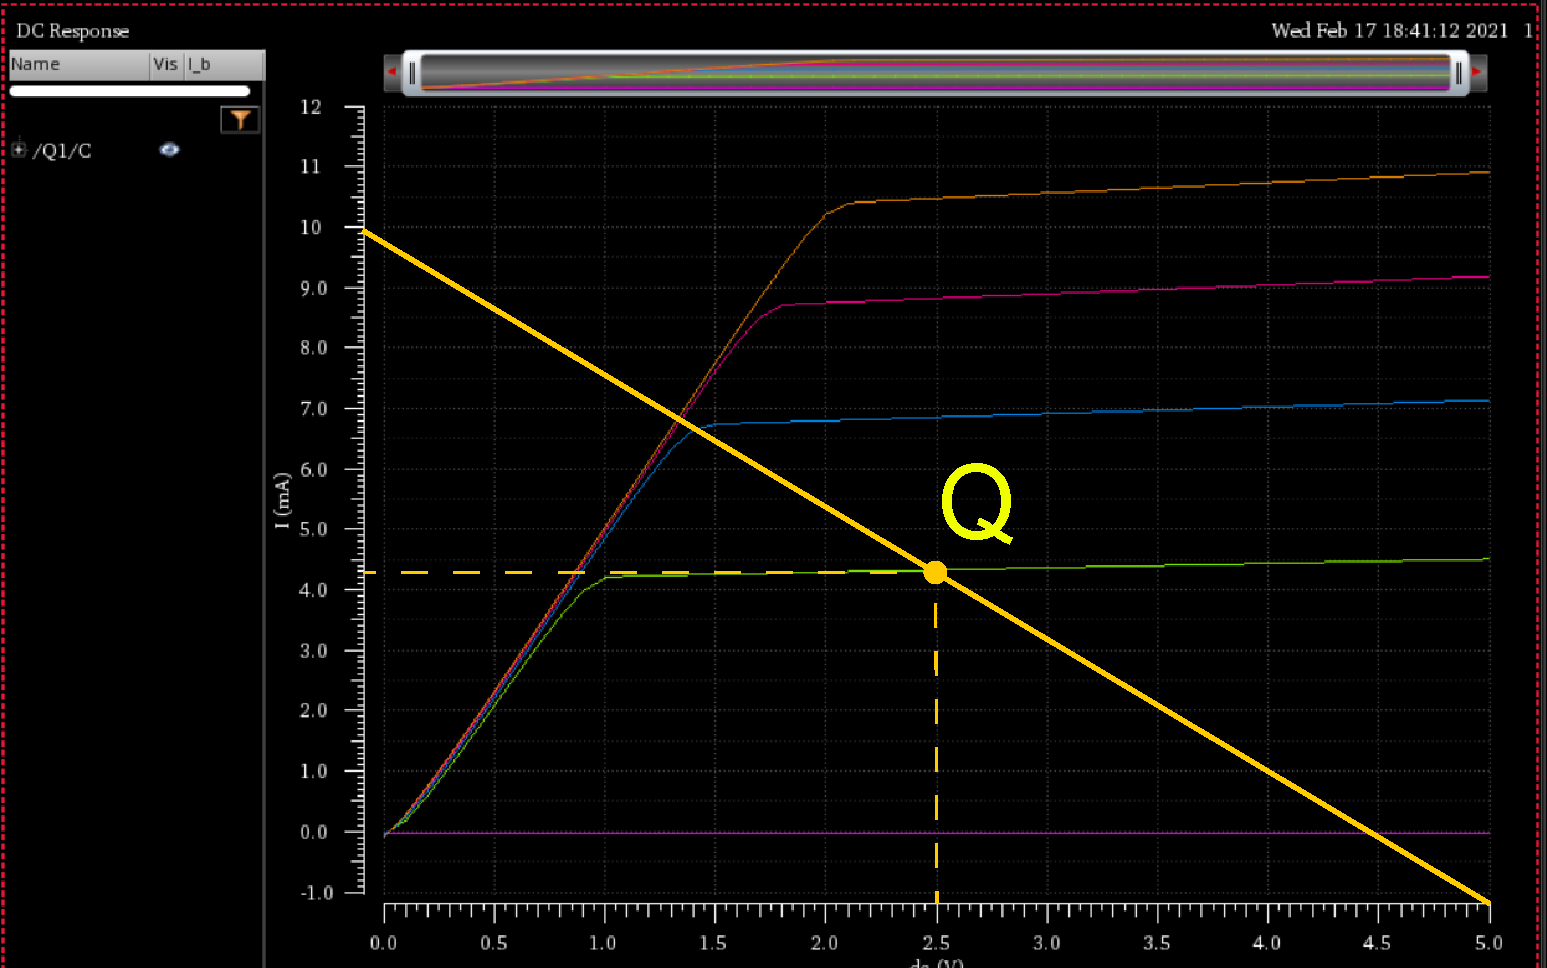
\includegraphics[width=0.6\linewidth]{1.png}}
\caption{Explanation to the consideration of the dynamics of elastic waves (a)
and an elastic stiffness matrix (b) for a cubic symmetry crystal.}
\label{ris1}
\end{figure}
\end{document}
